\documentclass[]{scrartcl}
\usepackage{amsmath}
\usepackage{amsfonts}
\usepackage{amssymb}
\usepackage{graphicx}
\usepackage{hyperref}
\usepackage[sharp]{easylist}
\usepackage{cleveref}
\usepackage{subcaption}
\usepackage{filecontents}
\usepackage[sort]{natbib}

\title{Theory: Linear elastoplasicity}
\author{Jean-Paul Pelteret}

\begin{filecontents}{\jobname.bib}
@Misc{Mergheim2018a,
  author =    {Julia Mergheim and Jean-Paul Pelteret and Ester Comellas},
  title =     {Lecture notes: Material Modelling and Simulation},
  year =      {2018},
  publisher = {Friedrich--Alexander Uniersit\"{a}t Erlangen--N\"{u}rnberg}
}
@Book{Simo2006a,
  title     = {Computational Inelasticity},
  publisher = {Springer Science \& Business Media},
  year      = {2000},
  author    = {Simo, J. C. and Hughes, Thomas J. R.},
  editor    = {Marsden, J. E. and Sirovich, L. and Wiggins, S.},
  volume    = {7},
  series    = {Interdisciplinary Applied Mathematics},
  isbn      = {978-0-387-97520-7},
  doi       = {10.1007/b98904},
}
\end{filecontents}

\begin{document}

\maketitle

\begin{abstract}
An introduction to the theory applied for elastoplasticity.
\end{abstract}

\section{Governing equations for quasi-static linear elasticity}
The strong statement of the balance of linear momentum reads
\begin{gather}
\nabla \cdot \boldsymbol{\sigma} + \mathbf{b} 
  = \mathbf{0}
\quad \text{on} \quad \Omega \quad ,
\end{gather}
where $\nabla = \frac{\partial}{\partial x}$ is a differential operator,
$\boldsymbol{\sigma}$ is the Cauchy stress tensor and
$\mathbf{b} = \rho \mathbf{g}$ is the body force density vector.
This is expressed in index notation as
\begin{gather}
\frac{\partial \sigma_{ij}}{\partial x_{j}} + b_{i} 
  = 0
\quad \text{on} \quad \Omega \quad .
\end{gather}
Pre-multiplying the above by test function $\delta \mathbf{v}$ and integrating over the domain $\Omega$ renders
\begin{gather}
- \int\limits_{\Omega} \delta v_{i} \,  \frac{\partial \sigma_{ij}}{\partial x_{j}} \, dv
  = \int\limits_{\Omega} \delta v_{i} \, b_{i} \, dv
\end{gather}
that, by using the product rule for derivatives (i.e. integration by parts), becomes
\begin{gather}
\int\limits_{\Omega} \frac{\partial \delta v_{i}}{\partial x_{j}} \, \sigma_{ij} \, dv
- \int\limits_{\Omega} \frac{\partial}{\partial x_{j}} \left[ \delta v_{i} \, \sigma_{ij} \right] \, dv
  = \int\limits_{\Omega} \delta v_{i} \, b_{i} \, dv
\quad .
\end{gather}
Finally, by applying divergence theorem to the second term in the above, we attain the weak form of the balance of linear momentum
\begin{gather}
\int\limits_{\Omega} \frac{\partial \delta v_{i}}{\partial x_{j}} \, \sigma_{ij} \, dv
  = \int\limits_{\Omega} \delta v_{i} \, b_{i} \, dv
  + \int\limits_{\partial\Omega} \delta v_{i} \, \underbrace{\sigma_{ij} \, n_{j}}_{\bar{t}_{i}} \, da
\quad ,
\label{equ: Weak form of the balance of linear momentum}
\end{gather}
wherein $\mathbf{n}$ represents the outward facing normal on $\partial\Omega$, the boundary of the domain, and $\bar{\mathbf{t}}$ the prescribed traction on the Neumann boundary.

\clearpage
\section{General framework for elastoplasticity}
\begin{easylist}[itemize]
# Kinematics
## Small strain tensor
\begin{gather}
\boldsymbol{\varepsilon} 
  = \frac{1}{2} \left[ \nabla \mathbf{u} + \left[ \nabla \mathbf{u} \right]^{T} \right]
  = \nabla\mathbf{u}^{sym}
\end{gather}
## Additive volumetric-isochoric split of the strain
\begin{gather}
\boldsymbol{\varepsilon} 
  = \boldsymbol{\varepsilon}^{vol} + \boldsymbol{\varepsilon}^{dev}
\quad ; \quad
\boldsymbol{\varepsilon}^{vol} = \dfrac{1}{3} \textrm{ tr}(\boldsymbol{\varepsilon}) \mathbf{I}
\end{gather}
## Additive split of strain into elastic and plastic contributions
\begin{gather*}
\boldsymbol{\varepsilon} 
  = \boldsymbol{\varepsilon}^{e} + \boldsymbol{\varepsilon}^{p}
\end{gather*}
# General free energy function
\begin{gather*}
\psi = \psi (\boldsymbol{\varepsilon}^{e}, \alpha, \boldsymbol{\beta})
\end{gather*}
## Two new internal variables:
### $\alpha$ describes the relative increase of the elastic region (isotropic hardening variable)
### $\boldsymbol{\beta}$ describes the kinematic hardening (a rank-2 tensor; related to the centre point of the elastic region and introduces anisotropy due to plastic flow)
# Principle of irreversibility: 
## Dissipation inequality
\begin{align*}
\mathcal{D} 
  &= \boldsymbol{\sigma} : \dot{\boldsymbol{\varepsilon}} - \dot\psi (\boldsymbol{\varepsilon}^{e}, \alpha, \boldsymbol{\beta}) \\
  &= \boldsymbol{\sigma} : \left[ \dot{\boldsymbol{\varepsilon}}^{e} + \dot{\boldsymbol{\varepsilon}}^{p} \right] 
  - \frac{\partial \psi}{\partial \boldsymbol{\varepsilon}^{e}} : \dot{\boldsymbol{\varepsilon}^{e}}
  \underbrace{- \frac{\partial \psi}{\partial \alpha}}_{R} \dot{\alpha}
  \underbrace{- \frac{\partial \psi}{\partial \boldsymbol{\beta}}}_{\boldsymbol{B}} : \dot{\boldsymbol{\beta}} \\ 
  &= \left[ \boldsymbol{\sigma} - \frac{\partial \psi}{\partial \boldsymbol{\varepsilon}^{e}} \right] : \dot{\boldsymbol{\varepsilon}^{e}}
  + \boldsymbol{\sigma} : \dot{\boldsymbol{\varepsilon}}^{p}
  + R \dot{\alpha}
  + \boldsymbol{B} : \dot{\boldsymbol{\beta}}
  \\
  &\geq 0
\end{align*}
### Hardening stress $R$
### Back stress $\boldsymbol{B}$
## Definition of Cauchy stress
\begin{gather}
\boldsymbol{\sigma} 
  := \frac{\partial \psi}{\partial \boldsymbol{\varepsilon}^{e}}
\end{gather}
## Reduced dissipation inequality (using definition of Cauchy stress)
\begin{gather*}
\mathcal{D}^{red}
  = \boldsymbol{\sigma} : \dot{\boldsymbol{\varepsilon}}^{p}
  + R \dot{\alpha}
  + \boldsymbol{B} : \dot{\boldsymbol{\beta}}
  \geq 0
\end{gather*}
# Evolution equations derived by the postulate of maximum dissipation [note: this ensures that hardening occurs when accommodated by the model, thus dissipating more energy than perfect plastic flow]
## Elastic region is restricted by yield function $\Phi \left( \boldsymbol{\sigma},R,\boldsymbol{B} \right)$:
\begin{gather}
\mathbb{E} := \left\lbrace \left( \boldsymbol{\sigma},R,\boldsymbol{B} \right) \vert \Phi \left( \boldsymbol{\sigma},R,\boldsymbol{B} \right) \leq 0 \right\rbrace
\end{gather}
## Conditions:
### Elastic state: $\Phi < 0$
### Plastic state: $\Phi = 0$
# Define Lagrange multiplier problem to maximise the dissipation, i.e.
\begin{gather*}
\textnormal{maximise } \mathcal{D}^{red} \textnormal{ subject to } \Phi \left( \boldsymbol{\sigma},R,\boldsymbol{B} \right) \leq 0 \\
\mathcal{L} \left( \boldsymbol{\sigma},R,\boldsymbol{B}, \dot{\lambda} \right)
  = -\mathcal{D}^{red} + \dot{\lambda} \Phi 
  \quad \rightarrow \quad \textnormal{stationary}
\end{gather*}
### $\dot{\lambda}$ is known as the consistency parameter
## Taking directional derivatives, we can identify the following evolution equations for the internal variables:
\begin{align*}
\frac{\partial \mathcal{L}}{\partial \boldsymbol{\sigma}} = \boldsymbol{0}
\quad &\Rightarrow \quad 
\dot{\boldsymbol{\varepsilon}}^{p} = \dot{\lambda} \frac{\partial \Psi}{\partial \boldsymbol{\sigma}}
\quad \textnormal{(flow rule)}
\\
\frac{\partial \mathcal{L}}{\partial R} = 0
\quad &\Rightarrow \quad 
\dot{\alpha} = \dot{\lambda} \frac{\partial \Psi}{\partial R}
\quad \textnormal{(evolution equation for isotropic hardening)}
\\
\frac{\partial \mathcal{L}}{\partial \boldsymbol{B}} = \boldsymbol{0}
\quad &\Rightarrow \quad
\dot{\boldsymbol{\beta}} = \dot{\lambda} \frac{\partial \Psi}{\partial \boldsymbol{B}}
\quad \textnormal{(evolution equation for kinematic hardening)}
\\
%\frac{\partial \mathcal{L}}{\partial \dot{\lambda}}
%  = \\
\end{align*}
% http://www.engr.colostate.edu/~thompson/hPage/CourseMat/Courses/CE696DV/plasticity.pdf
%https://www.ethz.ch/content/dam/ethz/special-interest/baug/ifb/ifb-dam/homepage-IfB/Education/msc_courses/msc-mechanics-building-materials/documents/plastizitaet.pdf
% p 36
## Loading / unloading condition:
\begin{align*}
\frac{\partial \Psi}{\partial \boldsymbol{\sigma}} \dot{\boldsymbol{\sigma}}
\begin{cases}
< 0 \quad & \textnormal{Unloading (elastic)} \\
= 0 \quad & \textnormal{Loading (plastic flow)} \\
> 0 \quad & \textnormal{Loading (plastic hardening)}
\end{cases}
%\textnormal{Loading (plastic hardening)}   &\frac{\partial \Psi}{\partial \boldsymbol{\sigma}} \dot{\boldsymbol{\sigma}} > 0 \\
%\textnormal{Loading (plastic flow): }   &\frac{\partial \Psi}{\partial \boldsymbol{\sigma}} \dot{\boldsymbol{\sigma}} = 0 \\
%\textnormal{Unloading: } &\frac{\partial \Psi}{\partial \boldsymbol{\sigma}} \dot{\boldsymbol{\sigma}} < 0
\end{align*}
### The loading-unloading conditions can be shown to be equivalent to the Karush-Kuhn-Tucker (KKT) conditions (an important statement in optimisation theory):
% https://en.wikipedia.org/wiki/Flow_plasticity_theory
% Simo, Computational elasticity, p77
\begin{gather}
\dot{\lambda} \geq 0
\quad;\quad
\Phi \leq 0
\quad;\quad
\dot{\lambda} \Phi = 0
\end{gather}
#### Situations and definitions for any $\left( \boldsymbol{\sigma},R,\boldsymbol{B} \right) \in \mathbb{E}$
\begin{align*}
\Phi < 0 
  \quad &\Rightarrow \quad 
  \left( \boldsymbol{\sigma},R,\boldsymbol{B} \right) \in \textnormal{int}(\mathbb{E})
  \quad \Rightarrow \quad 
  \dot{\lambda} = 0 \quad \textnormal{(Elastic response)} \\
\Phi = 0
  \quad &\Rightarrow \quad 
  \left( \boldsymbol{\sigma},R,\boldsymbol{B} \right) \in \partial\mathbb{E}
  \quad \Rightarrow \quad
  \begin{cases}
  \dot{\Phi} < 0 \quad \Rightarrow \quad \dot{\lambda} = 0 \quad  \textnormal{(Elastic unloading)} \\
  \dot{\Phi} = 0 \quad \textnormal{and} \quad \dot{\lambda} = 0 \quad  \textnormal{(Neutral loading)} \\
  \dot{\Phi} = 0 \quad \textnormal{and} \quad \dot{\lambda} > 0 \quad  \textnormal{(Plastic loading)}
  \end{cases}
\end{align*}
## Hardening / softening condition:
\begin{align*}
\frac{\partial \Psi}{\partial \alpha} \dot{\alpha}
\begin{cases}
< 0 \quad & \textnormal{Softening} \\
> 0 \quad & \textnormal{Hardening}
\end{cases}
%\textnormal{Softening: }   &\frac{\partial \Psi}{\partial \alpha} \dot{\alpha} > 0 \\
%\textnormal{Hardening: } &\frac{\partial \Psi}{\partial \alpha} \dot{\alpha} < 0
\end{align*}
# Example of Von-Mises yield criterion
## Convex yield surface defined by
\begin{gather*}
\Phi \left( \boldsymbol{\sigma} \right)
 = \sqrt{\frac{3}{2}} \Vert \boldsymbol{\sigma}^{dev} \Vert - \sigma_{y} 
 \leq 0
\end{gather*}
### Cylindrical yield-surface as observed in the principal stress space
### Norm of deviatoric stress contribution:
\begin{gather*}
\Vert \boldsymbol{\sigma}^{dev} \Vert
  = \sqrt{\boldsymbol{\sigma}^{dev} : \boldsymbol{\sigma}^{dev}}
\end{gather*}
\end{easylist}

\clearpage
\section{Constitutive law: Linear elasticity}

\begin{easylist}[itemize]
# Linear elasticity (a special case of hyperelasticity)
## Dissipation (in-)equality
\begin{gather}
\mathcal{D} 
  = \boldsymbol{\sigma} : \dot{\boldsymbol{\varepsilon}} - \dot\psi \left( \boldsymbol{\varepsilon} \right) 
  = 0
\quad \Rightarrow \quad
\boldsymbol{\sigma} 
  = \frac{\partial \psi \left( \boldsymbol{\varepsilon} \right)}{\partial \boldsymbol{\varepsilon}}
\end{gather}
## Free/Strain energy function (Hooke's law)
\begin{gather}
\psi(\boldsymbol{\varepsilon})
  = \dfrac{\lambda}{2} \left[\textrm{tr}(\boldsymbol{\varepsilon})\right]^2 
  + \mu \textrm{ tr}(\boldsymbol{\varepsilon}^2)
\end{gather}
## Cauchy stress
\begin{gather}
\boldsymbol{\sigma}(\boldsymbol{\varepsilon}) =  \dfrac{\partial \psi}{\partial \boldsymbol{\varepsilon}} = \lambda \textrm{ tr}(\boldsymbol{\varepsilon}) \mathbf{I} + 2\mu\boldsymbol{\varepsilon}
\end{gather}
## Elastic tangent
\begin{gather}
\mathbb{C} = \dfrac{{\partial}^2 \psi}{\partial \boldsymbol{\varepsilon}^2}: \dot{\boldsymbol{\varepsilon}} = \lambda \mathbf{I} \otimes \mathbf{I} + 2\mu\;\mathbb{I}^{sym}
\end{gather}
### with the linear relationship
\begin{gather}
\boldsymbol{\sigma}
  = \boldsymbol{\mathbb{C}} : \boldsymbol{\varepsilon}
\end{gather}
\end{easylist}

\clearpage
\section{Constitutive law: Elastoplasticity}

The linear elastoplastic constitutive laws and framework described here are described in detail by \citep{Simo2006a,Mergheim2018a}.

\subsection{Associated Von Mises elastoplasticity with linear isotropic and kinematic hardening}
\begin{easylist}
# Kinematics
\begin{gather*}
\varepsilon
  = \varepsilon^{e} + \varepsilon^{p}
\end{gather*}
# Free energy (additive decomposition into elastic and plastic parts)
\begin{align*}
\psi (\boldsymbol{\varepsilon}^{e}, \alpha, \boldsymbol{\beta})
 &= \psi^{e} (\boldsymbol{\varepsilon}^{e})
  + \psi^{p} (\alpha, \boldsymbol{\beta}) \\
\psi^{e} (\boldsymbol{\varepsilon}^{e})
 &= \frac{\lambda}{2} \left[ \textnormal{tr} (\boldsymbol{\varepsilon}^{e}) \right]^{2} 
   + \mu \textnormal{tr} \left( \left[\boldsymbol{\varepsilon}^{e} \right]^{2} \right) \\  
\psi^{p} (\alpha, \boldsymbol{\beta})
 &= \frac{1}{2} k r \alpha^{2} + \frac{1}{2} k \left[ 1 - r \right] \Vert \boldsymbol{\beta} \Vert^{2}
 \quad , \quad r \in \left[ 0,1 \right]
\end{align*}
# Stresses
\begin{align*}
\boldsymbol{\sigma} 
 &=  \dfrac{\partial \psi}{\partial \boldsymbol{\varepsilon^{e}}} 
  = \lambda \textrm{ tr}(\boldsymbol{\varepsilon}^{e}) \mathbf{1} + 2\mu\boldsymbol{\varepsilon}^{e} \\
R 
 &= - \dfrac{\partial \psi}{\partial \alpha}
  = - k r \alpha \\
\boldsymbol{B}
 &= - \dfrac{\partial \psi}{\partial \boldsymbol{\beta}}
  = -k \left[ 1 - r \right] \boldsymbol{\beta}
\end{align*}
# Yield function (Von Mises)
\begin{gather*}
\Phi \left( \boldsymbol{\sigma},R,\boldsymbol{B} \right)
  = \Vert \boldsymbol{\sigma}^{dev} + \boldsymbol{B} \Vert - \sqrt{\frac{2}{3}} \left[ \sigma_{y} - R \right]
  \leq 0
\end{gather*}
# Evolution equations
\begin{align*}
\dot{\boldsymbol{\varepsilon}}^{p} 
 &= \dot{\lambda} \frac{\partial \Phi}{\partial \boldsymbol{\sigma}}
  = \dot{\lambda} \dfrac{\boldsymbol{\sigma}^{dev} + \boldsymbol{B}}{\Vert \boldsymbol{\sigma}^{dev} + \boldsymbol{B} \Vert}
  = \dot{\lambda} \boldsymbol{n}
\\
\dot{\alpha} 
 &= \dot{\lambda} \frac{\partial \Phi}{\partial R}
  = \sqrt{\frac{2}{3}} \dot{\lambda}
\\
\dot{\boldsymbol{\beta}} 
 &= \dot{\lambda} \frac{\partial \Phi}{\partial \boldsymbol{B}}
  = \dot{\lambda} \dfrac{\boldsymbol{\sigma}^{dev} + \boldsymbol{B}}{\Vert \boldsymbol{\sigma}^{dev} + \boldsymbol{B} \Vert}
  = \dot{\lambda} \boldsymbol{n}
\end{align*}
## Must satisfy KTT conditions
\begin{gather*}
\dot{\lambda} \geq 0
\quad;\quad
\Phi \leq 0
\quad;\quad
\dot{\lambda} \Phi = 0
\end{gather*}
# Principle of irreversibility
\begin{align*}
\mathcal{D}^{red}
 &= \boldsymbol{\sigma} : \dot{\boldsymbol{\varepsilon}}^{p}
  + R \dot{\alpha}
  + \boldsymbol{B} : \dot{\boldsymbol{\beta}} \\
 &= \boldsymbol{\sigma} : \dot{\lambda} \boldsymbol{n}
   + R \sqrt{\frac{2}{3}} \dot{\lambda}
   + \boldsymbol{B} : \dot{\lambda} \boldsymbol{n} \\
 &= \dot{\lambda} \left[ \left[ 
    \boldsymbol{\sigma} + \boldsymbol{B} \right] : \boldsymbol{n}
   + R \sqrt{\frac{2}{3}}
   \right] \\
 &= \dot{\lambda} \left[ \left[ 
    \boldsymbol{\sigma}^{dev} + \boldsymbol{B} \right] : \dfrac{\boldsymbol{\sigma}^{dev} + \boldsymbol{B}}{\Vert \boldsymbol{\sigma}^{dev} + \boldsymbol{B} \Vert}
   + R \sqrt{\frac{2}{3}}
   \right] \\
 &= \dot{\lambda} \left[ \
    \Vert \boldsymbol{\sigma}^{dev} + \boldsymbol{B} \Vert
   + R \sqrt{\frac{2}{3}}
   \right] \\
 &\geq 0
\end{align*}
## If $\Phi < 0 \quad \Rightarrow \quad \dot{\lambda} = 0$
## If $\Phi = 0 \quad \Rightarrow \quad \dot{\lambda} > 0$ 
   and $\Vert \boldsymbol{\sigma}^{dev} + \boldsymbol{B} \Vert + R \sqrt{\dfrac{2}{3}} = \sqrt{\dfrac{2}{3}} \sigma_{y} \geq 0$
# Consistency condition (evolution of yield surface)
\begin{align*}
\dot{\Phi}
 &= \frac{\partial \Phi}{\partial \boldsymbol{\sigma}} : \dot{\boldsymbol{\sigma}}
  + \frac{\partial \Phi}{\partial R} \dot{R}
  + \frac{\partial \Phi}{\partial \boldsymbol{B}} : \dot{\boldsymbol{B}} \\
 &= \frac{\partial \Phi}{\partial \boldsymbol{\sigma}} : \dfrac{\partial^{2} \psi}{\partial \boldsymbol{\varepsilon^{e}} \otimes \partial \boldsymbol{\varepsilon^{e}}} : \underbrace{ \left[ \dot{\boldsymbol{\varepsilon}} - \dot{\boldsymbol{\varepsilon^{p}}} \right]}_{\dot{\boldsymbol{\varepsilon^{e}}}}
  - \frac{\partial \Phi}{\partial R} \dfrac{\partial^{2} \psi}{\partial \alpha \partial \alpha} \dot{\alpha}
  - \frac{\partial \Phi}{\partial \boldsymbol{B}} : \dfrac{\partial^{2} \psi}{\partial \boldsymbol{\beta} \otimes \partial \boldsymbol{\beta}} : \dot{\boldsymbol{\beta}} \\
% &= \frac{\partial \Phi}{\partial \boldsymbol{\sigma}} : \dfrac{\partial^{2} \psi}{\partial \boldsymbol{\varepsilon^{e}} \otimes \partial \boldsymbol{\varepsilon^{e}}} : \dot{\boldsymbol{\varepsilon}} 
%  - \frac{\partial \Phi}{\partial \boldsymbol{\sigma}} : \dfrac{\partial^{2} \psi}{\partial \boldsymbol{\varepsilon^{e}} \otimes \partial \boldsymbol{\varepsilon^{e}}} : \dot{\boldsymbol{\varepsilon^{p}}}
%  - \frac{\partial \Phi}{\partial R} \dfrac{\partial^{2} \psi}{\partial \alpha \partial \alpha} \dot{\alpha}
%  - \frac{\partial \Phi}{\partial \boldsymbol{B}} : \dfrac{\partial^{2} \psi}{\partial \boldsymbol{\beta} \otimes \partial \boldsymbol{\beta}} : \dot{\boldsymbol{\beta}} \\
 &= \frac{\partial \Phi}{\partial \boldsymbol{\sigma}} : \dfrac{\partial^{2} \psi}{\partial \boldsymbol{\varepsilon^{e}} \otimes \partial \boldsymbol{\varepsilon^{e}}} : \dot{\boldsymbol{\varepsilon}} 
  - \frac{\partial \Phi}{\partial \boldsymbol{\sigma}} : \dfrac{\partial^{2} \psi}{\partial \boldsymbol{\varepsilon^{e}} \otimes \partial \boldsymbol{\varepsilon^{e}}} : \frac{\partial \Phi}{\partial \boldsymbol{\sigma}} \dot{\lambda}
  - \frac{\partial \Phi}{\partial R} \dfrac{\partial^{2} \psi}{\partial \alpha \partial \alpha} \frac{\partial \Phi}{\partial R} \dot{\lambda}
  - \frac{\partial \Phi}{\partial \boldsymbol{B}} : \dfrac{\partial^{2} \psi}{\partial \boldsymbol{\beta} \otimes \partial \boldsymbol{\beta}} : \frac{\partial \Phi}{\partial \boldsymbol{B}}  \dot{\lambda} \\
 &= \frac{\partial \Phi}{\partial \boldsymbol{\sigma}} : \dfrac{\partial^{2} \psi}{\partial \boldsymbol{\varepsilon^{e}} \otimes \partial \boldsymbol{\varepsilon^{e}}} : \dot{\boldsymbol{\varepsilon}} 
  -  \dot{\lambda} \left[ 
  \frac{\partial \Phi}{\partial \boldsymbol{\sigma}} : \dfrac{\partial^{2} \psi}{\partial \boldsymbol{\varepsilon^{e}} \otimes \partial \boldsymbol{\varepsilon^{e}}} : \frac{\partial \Phi}{\partial \boldsymbol{\sigma}}
  + \frac{\partial \Phi}{\partial R} \dfrac{\partial^{2} \psi}{\partial \alpha \partial \alpha} \frac{\partial \Phi}{\partial R}
  + \frac{\partial \Phi}{\partial \boldsymbol{B}} : \dfrac{\partial^{2} \psi}{\partial \boldsymbol{\beta} \otimes \partial \boldsymbol{\beta}} : \frac{\partial \Phi}{\partial \boldsymbol{B}}
  \right] \\
 &= 0 \quad \textnormal{(stay on yield surface during plastic deformation)}
\end{align*}
\begin{align*}
\Rightarrow \quad \dot{\lambda}
  = \dfrac { \dfrac{\partial \Phi}{\partial \boldsymbol{\sigma}} : \dfrac{\partial^{2} \psi}{\partial \boldsymbol{\varepsilon^{e}} \otimes \partial \boldsymbol{\varepsilon^{e}}} : \dot{\boldsymbol{\varepsilon}}  }{ \dfrac{\partial \Phi}{\partial \boldsymbol{\sigma}} : \dfrac{\partial^{2} \psi}{\partial \boldsymbol{\varepsilon^{e}} \otimes \partial \boldsymbol{\varepsilon^{e}}} : \dfrac{\partial \Phi}{\partial \boldsymbol{\sigma}}
    + \dfrac{\partial \Phi}{\partial R} \dfrac{\partial^{2} \psi}{\partial \alpha \partial \alpha} \dfrac{\partial \Phi}{\partial R}
    + \dfrac{\partial \Phi}{\partial \boldsymbol{B}} : \dfrac{\partial^{2} \psi}{\partial \boldsymbol{\beta} \otimes \partial \boldsymbol{\beta}} : \dfrac{\partial \Phi}{\partial \boldsymbol{B}} }
\end{align*}
with
\begin{align*}
\dfrac{\partial^{2} \psi}{\partial \boldsymbol{\varepsilon^{e}} \otimes \partial \boldsymbol{\varepsilon^{e}}}
 &= \mathbb{C} \\
\dfrac{\partial^{2} \psi}{\partial \alpha \partial \alpha}
 &= -k r \\
\dfrac{\partial^{2} \psi}{\partial \boldsymbol{\beta} \otimes \partial \boldsymbol{\beta}}
 &= -k \left[ 1-r \right] \mathbb{I}^{sym} \\
\dfrac{\partial \Phi}{\partial \boldsymbol{\sigma}}
 &= \dfrac{\partial \Vert \boldsymbol{\sigma}^{dev} + \boldsymbol{B} \Vert}{\partial \left( \boldsymbol{\sigma}^{dev} + \boldsymbol{B} \right)} : \dfrac{\partial \left( \boldsymbol{\sigma}^{dev} + \boldsymbol{B} \right)}{\partial \boldsymbol{\sigma}}
  = \dfrac{\boldsymbol{\sigma}^{dev} + \boldsymbol{B}}{\Vert \boldsymbol{\sigma}^{dev} + \boldsymbol{B} \Vert} : \mathbb{I}^{sym}
  = \boldsymbol{n} \\
\dfrac{\partial \Phi}{\partial R}
 &= \sqrt{\frac{2}{3}} \\
\dfrac{\partial \Phi}{\partial \boldsymbol{B}}
 &= \boldsymbol{n}
\end{align*}
Then
\begin{align*}
\Rightarrow \quad \dot{\lambda}
 &= \dfrac { \boldsymbol{n} : \mathbb{C} : \dot{\boldsymbol{\varepsilon}}  }{ \boldsymbol{n} : \mathbb{C} : \boldsymbol{n}
    + \sqrt{\frac{2}{3}} \left[ -k r \right] \sqrt{\frac{2}{3}}
    + \boldsymbol{n} : \left[ -k \left[ 1-r \right] \mathbb{I}^{sym} \right] : \boldsymbol{n} } \\
 &= \dfrac { \boldsymbol{n} : \mathbb{C} : \dot{\boldsymbol{\varepsilon}}  }{ \boldsymbol{n} : \mathbb{C} : \boldsymbol{n}
    - \frac{2}{3} k r
    -k \left[ 1-r \right] } \\
 &= \dfrac { \boldsymbol{n} : \mathbb{C} : \dot{\boldsymbol{\varepsilon}}  }{ \boldsymbol{n} : \mathbb{C} : \boldsymbol{n}
    + k \left[\frac{1}{3} r - 1 \right] } \\
\end{align*}
\end{easylist}

\subsection{Elasto-plastic tangent modulus (continuous setting)}
\begin{easylist}
# Goal
\begin{gather*}
\dot{\boldsymbol{\sigma}} 
  = \boldsymbol{\mathcal{C}}^{ep} : \dot{\boldsymbol{\varepsilon}}
\end{gather*}
# Stress rate
\begin{gather*}
\boldsymbol{\sigma}
  = \frac{\partial \Psi}{\partial \boldsymbol{\varepsilon}^{e}} \\
\Rightarrow \quad
\dot{\boldsymbol{\sigma}}
  = \frac{\partial^{2} \Psi}{\partial \boldsymbol{\varepsilon}^{e} \otimes \partial \boldsymbol{\varepsilon}^{e}} : \dot{\boldsymbol{\varepsilon}}^{e}
  = \boldsymbol{\mathcal{C}} : \left[ \dot{\boldsymbol{\varepsilon}} - \dot{\boldsymbol{\varepsilon}}^{p} \right]
  = \boldsymbol{\mathcal{C}} : \left[ \dot{\boldsymbol{\varepsilon}} - \dot{\lambda} \frac{\partial \Phi}{\partial \boldsymbol{\sigma}} \right]
\end{gather*}
# Remember: Plastic potential $\Phi \left( \boldsymbol{\sigma},\boldsymbol{S} \right)$ with evolution laws
$
\dot{\boldsymbol{\varepsilon}}^{p} 
  = \dot{\lambda} \dfrac{\partial \Phi}{\partial \boldsymbol{\sigma}}
$, $
\dot{\boldsymbol{d}} 
  = \dot{\lambda} \dfrac{\partial \Phi}{\partial \boldsymbol{S}}
$
## Definition and derivatives of stress-like terms $\boldsymbol{S} = \left[ R,\boldsymbol{B} \right]$ with internal variables $\boldsymbol{d} = \left[ \alpha,\boldsymbol{\beta} \right]$
\begin{gather*}
\boldsymbol{S} 
  = - \frac{\partial \Psi}{\partial \boldsymbol{d}} \\
\dot{\boldsymbol{S}} 
  = - \frac{\partial^{2} \Psi}{\partial \boldsymbol{d} \otimes \partial \boldsymbol{d}} \circ \dot{\boldsymbol{d}}
  =  - \frac{\partial^{2} \Psi}{\partial \boldsymbol{d} \otimes \partial \boldsymbol{d}} \circ \dot{\lambda} \frac{\partial \Phi}{\partial \boldsymbol{S}} \\
\end{gather*}
# Use consistency condition to compute $\dot{\lambda}$:
\begin{gather*}
\dot{\lambda} \dot{\Phi} = 0 
\quad \Rightarrow  \quad
\dot{\Phi} = 0 \quad \textnormal{for plastic loading}
\end{gather*}
\begin{align*}
\dot{\Phi}
 &= \frac{\partial \Phi}{\partial \boldsymbol{\sigma}} : \dot{\boldsymbol{\sigma}}
  + \frac{\partial \Phi}{\partial \boldsymbol{S}} \circ \dot{\boldsymbol{S}} \\
 &= \frac{\partial \Phi}{\partial \boldsymbol{\sigma}} : \boldsymbol{\mathcal{C}} : \left[ \dot{\boldsymbol{\varepsilon}} - \dot{\lambda} \frac{\partial \Phi}{\partial \boldsymbol{\sigma}} \right]
  -  \frac{\partial \Phi}{\partial \boldsymbol{S}} \circ \frac{\partial^{2} \Psi}{\partial \boldsymbol{d} \otimes \partial \boldsymbol{d}} \circ \dot{\lambda} \frac{\partial \Phi}{\partial \boldsymbol{S}} \\
 &= 0 \\
\Rightarrow \quad 
\dot{\lambda}
  &= \frac{1}{D} \frac{\partial \Phi}{\partial \boldsymbol{\sigma}} : \boldsymbol{\mathcal{C}} : \dot{\boldsymbol{\varepsilon}}
\quad \textnormal{with} \\
D 
  &= \frac{\partial \Phi}{\partial \boldsymbol{\sigma}} : \boldsymbol{\mathcal{C}} : \frac{\partial \Phi}{\partial \boldsymbol{\sigma}}
  + \frac{\partial \Phi}{\partial \boldsymbol{S}} \circ \frac{\partial^{2} \Psi}{\partial \boldsymbol{d} \otimes \partial \boldsymbol{d}} \circ \frac{\partial \Phi}{\partial \boldsymbol{S}}
\end{align*}
# Elasto-plastic tangent
\begin{gather*}
\dot{\boldsymbol{\sigma}} 
  = \boldsymbol{\mathcal{C}}^{ep} : \dot{\boldsymbol{\varepsilon}}
  = \underbrace{\left[ \boldsymbol{\mathcal{C}} - \frac{1}{D} \left[ \boldsymbol{\mathcal{C}} : \frac{\partial \Phi}{\partial \boldsymbol{\sigma}} \right] \otimes \left[ \frac{\partial \Phi}{\partial \boldsymbol{\sigma}} : \boldsymbol{\mathcal{C}} \right] \right]}_{\boldsymbol{\mathcal{C}}^{ep} \textnormal{ (symmetric)}} : \dot{\boldsymbol{\varepsilon}}
\end{gather*}
# Result for isotropic hardening
\begin{subequations}
\begin{align}
\boldsymbol{\mathcal{C}}^{ep, dev}
 &= 2 \mu \boldsymbol{\mathcal{I}}^{dev} - \frac{\left[ 2\mu \right]^{2}}{2\mu + \frac{2}{3}k} \boldsymbol{n} \otimes \boldsymbol{n} \\
\boldsymbol{\mathcal{C}}^{ep, vol}
 &= \kappa \boldsymbol{1} \otimes \boldsymbol{1}
 \label{equ: Constutitve law: Algorithmically correct tangent: Volumetric}
\end{align}
\end{subequations}
with
\begin{gather*}
\boldsymbol{n}
  = \frac{\boldsymbol{\sigma}^{dev}}{\Vert \boldsymbol{\sigma}^{dev} \Vert}
\end{gather*}
\end{easylist}

\section{Integration algorithms for elasto-plasticity}
\subsection{Radial return algorithm for von Mises plasticity with linear isotropic hardening}
\begin{easylist}
# Constitutive setting
\begin{gather*}
\boldsymbol{\varepsilon}
  = \boldsymbol{\varepsilon}^{e} + \boldsymbol{\varepsilon}^{p}
  = \boldsymbol{\varepsilon}^{vol} + \boldsymbol{\varepsilon}^{dev} 
\\
\psi
  = \frac{1}{2} \kappa \left[ \textnormal{tr} \left( \boldsymbol{\varepsilon}^{vol} \right) \right]^{2}
  + \mu \textnormal{tr} \left( \left[\boldsymbol{\varepsilon}^{e, dev} \right]^{2} \right)
  + \frac{1}{2} k  \alpha^{2} 
\\
\Phi \left( \boldsymbol{\sigma}, R \right)
  = \Vert \boldsymbol{\sigma}^{dev} \Vert - \sqrt{\frac{2}{3}} \left[ \sigma_{y} - R \right]
    \leq 0
\\
\dot{\boldsymbol{\varepsilon}}^{p} 
  = \dot{\lambda} \frac{\partial \Phi}{\partial \boldsymbol{\sigma}}
%  = \dot{\lambda} \dfrac{\boldsymbol{\sigma}^{dev}}{\Vert \boldsymbol{\sigma}^{dev} \Vert}
  = \dot{\lambda} \boldsymbol{n}
\quad , \quad
\boldsymbol{n}
  = \dfrac{\boldsymbol{\sigma}^{dev}}{\Vert \boldsymbol{\sigma}^{dev} \Vert}
\\
\dot{\alpha} 
  = \dot{\lambda} \frac{\partial \Phi}{\partial R}
  = \sqrt{\frac{2}{3}} \dot{\lambda}
\end{gather*}
# Apply backward Euler method to evolution equations
\begin{gather*}
\boldsymbol{\varepsilon}^{p}_{n+1}
  = \boldsymbol{\varepsilon}^{p}_{n}
  + \Delta t \, \dot{\boldsymbol{\varepsilon}}^{p}_{n+1}
  = \boldsymbol{\varepsilon}^{p}_{n}
  + \Delta t \, \dot{\lambda}_{n+1} \boldsymbol{n}_{n+1}
\\ 
\alpha_{n+1}
  = \alpha_{n}
  + \Delta t \, \dot{\alpha}_{n+1}
  = \alpha_{n}
  + \Delta t \, \dot{\lambda}_{n+1} \sqrt{\frac{2}{3}}
\end{gather*}
# Deviatoric stress
\begin{align*}
\boldsymbol{\sigma}^{dev}_{n+1}
 & = 2 \mu \boldsymbol{\varepsilon}^{e, dev}_{n+1}
  = 2 \mu \left[ \boldsymbol{\varepsilon}^{dev}_{n+1} - \boldsymbol{\varepsilon}^{p, dev}_{n+1} \right] \\
 &= 2 \mu  \boldsymbol{\varepsilon}^{dev}_{n+1} 
  - 2 \mu \left[ \boldsymbol{\varepsilon}^{p}_{n}
  + \Delta t \, \dot{\lambda}_{n+1} \boldsymbol{n}_{n+1} \right] \\
% &= \underbrace{2 \mu \left[ \boldsymbol{\varepsilon}^{dev} - \boldsymbol{\varepsilon}^{p}_{n} \right]}_{\boldsymbol{\sigma}^{dev, trial}_{n+1}}
%  - 2 \mu \Delta t \, \dot{\lambda}_{n+1} \boldsymbol{n}_{n+1} \\
 &= \underbrace{2 \mu \left[ \boldsymbol{\varepsilon}^{dev}_{n+1} - \boldsymbol{\varepsilon}^{p}_{n} \right]}_{\boldsymbol{\sigma}^{dev, trial}_{n+1}}
  - 2 \mu \Delta \lambda_{n+1} \dfrac{\boldsymbol{\sigma}^{dev}_{n+1}}{\Vert \boldsymbol{\sigma}^{dev}_{n+1} \Vert} 
\quad (\textnormal{Note: } \Delta t \, \dot{\lambda}_{n+1} = \Delta \lambda_{n+1})
%\\
%\Rightarrow \quad
%\boldsymbol{\sigma}^{dev, trial}_{n+1}
% &= \left[ 1 + \dfrac{2 \mu \Delta \lambda_{n+1}}{\Vert \boldsymbol{\sigma}^{dev}_{n+1} \Vert} \right] \boldsymbol{\sigma}^{dev}_{n+1} 
\\
\Rightarrow \quad
\boldsymbol{\sigma}^{dev}_{n+1}
 &= \left[ 1 + \dfrac{2 \mu \Delta \lambda_{n+1}}{\Vert \boldsymbol{\sigma}^{dev}_{n+1} \Vert} \right]^{-1} \boldsymbol{\sigma}^{dev, trial}_{n+1} 
\end{align*}
\clearpage
### The final stress state is obtained by projecting the trial stress state onto the current yield surface.
\begin{figure}[!htb]
\centering
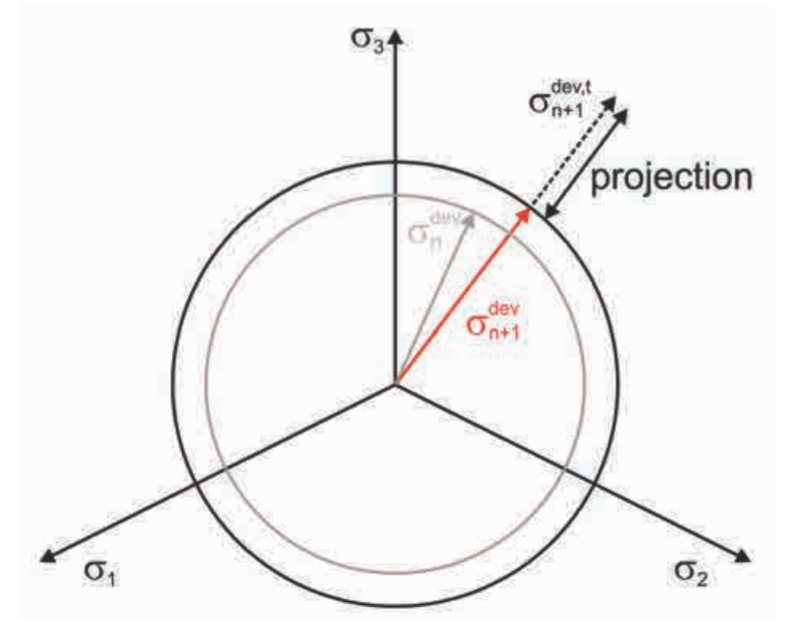
\includegraphics[width=0.7\linewidth]{Figures/Sec_3_5_1-Radial_projection}
\caption{Radial projection \citep{Mergheim2018a}}
\label{fig:sec351-radialprojection}
\end{figure}
## Still need to determine $\Vert \boldsymbol{\sigma}^{dev}_{n+1} \Vert$. Use coaxiality of the stresses:
\begin{gather*}
\dfrac{\boldsymbol{\sigma}^{dev, trial}_{n+1}}{\Vert \boldsymbol{\sigma}^{dev, trial}_{n+1} \Vert}
  = \dfrac{\boldsymbol{\sigma}^{dev}_{n+1}}{\Vert \boldsymbol{\sigma}^{dev}_{n+1} \Vert}
  = \boldsymbol{n}_{n+1}
\end{gather*}
### Contract both sides of previous equation by $\boldsymbol{n}_{n+1}$ and use definition of tensor norm $\Vert \boldsymbol{\sigma} \Vert$:
\begin{gather*}
\boldsymbol{\sigma}^{dev}_{n+1} : \dfrac{\boldsymbol{\sigma}^{dev}_{n+1}}{\Vert \boldsymbol{\sigma}^{dev}_{n+1} \Vert}
  = \boldsymbol{\sigma}^{dev, trial}_{n+1} : \dfrac{\boldsymbol{\sigma}^{dev, trial}_{n+1}}{\Vert \boldsymbol{\sigma}^{dev, trial}_{n+1} \Vert}
  - 2 \mu \Delta \lambda_{n+1} \dfrac{\boldsymbol{\sigma}^{dev}_{n+1}}{\Vert \boldsymbol{\sigma}^{dev}_{n+1} \Vert} : \dfrac{\boldsymbol{\sigma}^{dev}_{n+1}}{\Vert \boldsymbol{\sigma}^{dev}_{n+1} \Vert} \\
\Rightarrow \quad
\Vert \boldsymbol{\sigma}^{dev}_{n+1} \Vert
  = \Vert \boldsymbol{\sigma}^{dev, trial}_{n+1} \Vert
  - 2 \mu \Delta \lambda_{n+1}
\end{gather*}
## Yield function (plastic flow: $\Phi = 0$)
\begin{gather*}
\Phi_{n+1}
  = \Vert \boldsymbol{\sigma}^{dev}_{n+1} \Vert - \sqrt{\frac{2}{3}} \left[ \sigma_{y} + \underbrace{k \alpha_{n+1}}_{- R_{n+1}} \right]
  = 0 \\
\Rightarrow \quad
\Vert \boldsymbol{\sigma}^{dev}_{n+1} \Vert
  = \sqrt{\frac{2}{3}} \left[ \sigma_{y} + k \left[ \alpha_{n} + \Delta \lambda_{n+1} \sqrt{\frac{2}{3}} \right] \right]
\end{gather*}
## Plastic multiplier update computed by equating the two above equations
\begin{gather*}
\Vert \boldsymbol{\sigma}^{dev}_{n+1} \Vert
  = \Vert \boldsymbol{\sigma}^{dev, trial}_{n+1} \Vert
  - 2 \mu \Delta \lambda_{n+1}
  = \sqrt{\frac{2}{3}} \left[ \sigma_{y} + k \left[ \alpha_{n} + \Delta \lambda_{n+1} \sqrt{\frac{2}{3}} \right] \right] \\
\Rightarrow \quad
\underbrace{\Vert \boldsymbol{\sigma}^{dev, trial}_{n+1} \Vert - \sqrt{\frac{2}{3}} \left[ \sigma_{y} + k \alpha_{n} \right]}_{\Phi^{trial}_{n+1}}
  = \Delta \lambda_{n+1} \left[ 2 \mu + \frac{2}{3} k \right] \\
\Rightarrow \quad
\Delta \lambda_{n+1}
  = \frac{\Phi^{trial}_{n+1}}{2 \mu + \frac{2}{3} k}
\end{gather*}
# Remarks
## Within ideal von Mises plasticity or with linear hardening, $\dot{\lambda}_{n+1}$ can be computed directly.
   Otherwise, $\Phi_{n+1}$ has to be solver iteratively for $\dot{\lambda}_{n+1}$ (e.g. using Newton's method)
## For general yield functions, the closest point projection is the extension of the radial return algorithm.
%# Algorithm
%## Show slides
\end{easylist}

\subsection{General closest-point projection (for general plasticity and hardening laws)}
\begin{easylist}
# Difference between radial and closest point projection
\begin{figure}[!htb]
\centering
\begin{subfigure}[t]{0.45\textwidth}
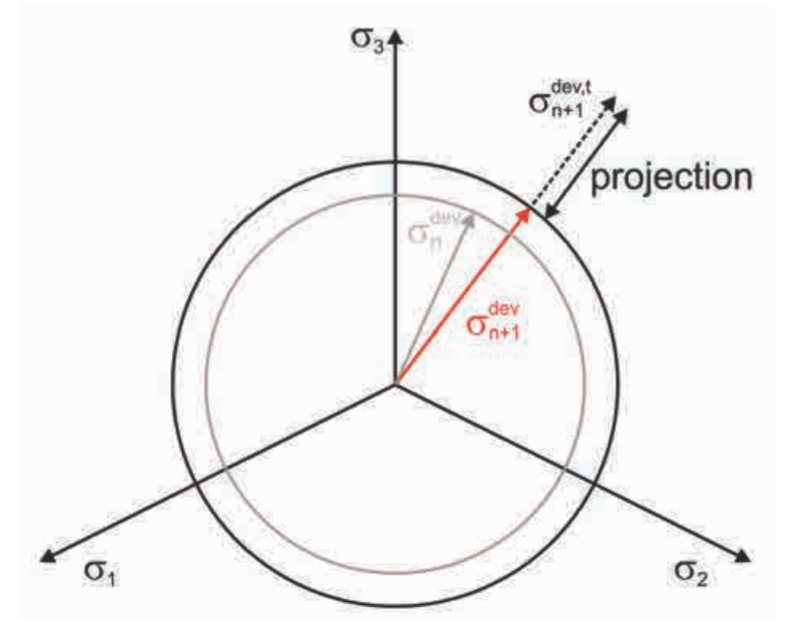
\includegraphics[width=0.8\linewidth]{Figures/Sec_3_5_1-Radial_projection}
\caption{Radial projection \citep{Mergheim2018a}}
\label{fig:sec351-radialprojection}
\end{subfigure}
\quad
\begin{subfigure}[t]{0.45\textwidth}
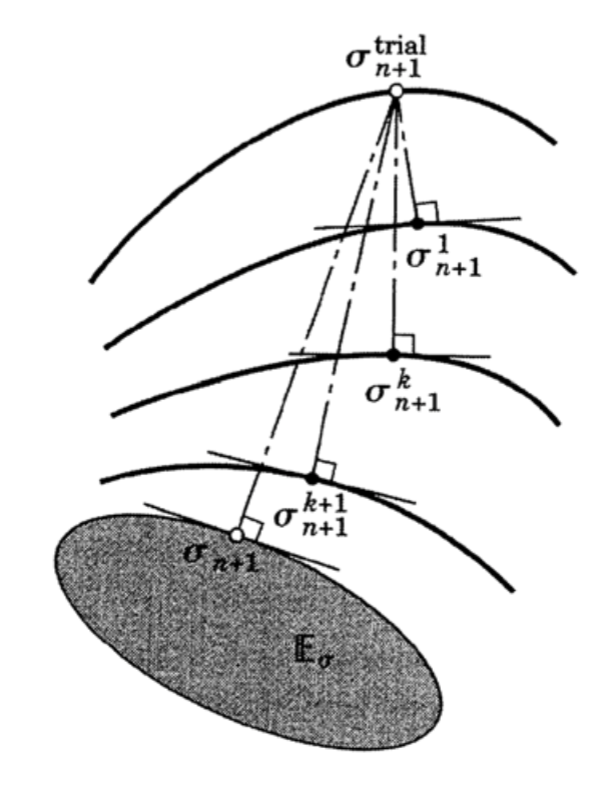
\includegraphics[width=0.8\linewidth]{Figures/Sec_3_5_2-General_closest_point_projection}
\caption{Closest-point projection \citep{Simo2006a}}
\label{fig:sec352-generalclosestpointprojection}
\end{subfigure}
\end{figure}
\end{easylist}

\subsection{Consistent elastoplastic tangent modulus for von Mises plasticity with only linear isotropic hardening (time discrete setting)}
\begin{easylist}
# Note: The definition of the consistent elastoplastic tangent depends on the algorithms used to update stresses, internal variables
# Goal: Tangent to compute
\begin{gather}
 \boldsymbol{\mathcal{C}}^{ep} 
  = \frac{\partial \boldsymbol{\sigma}_{n+1}}{\partial \boldsymbol{\varepsilon}_{n+1}}
  = \boldsymbol{\mathcal{C}}^{ep, vol} + \boldsymbol{\mathcal{C}}^{ep, dev}
\label{equ: Constutitve law: Algorithmically correct tangent}
\end{gather}
# Stress tensors
\begin{gather*}
\boldsymbol{\sigma}_{n+1}
  = \boldsymbol{\sigma}^{vol}_{n+1} + \boldsymbol{\sigma}^{dev}_{n+1} \\
\boldsymbol{\sigma}^{vol}_{n+1}
  = \kappa \boldsymbol{\varepsilon}^{vol}_{n+1} \\
\boldsymbol{\sigma}^{dev}_{n+1}
  = \boldsymbol{\sigma}^{dev, trial}_{n+1}
  - 2 \mu \Delta \lambda_{n+1} \boldsymbol{n}_{n+1} \\
\boldsymbol{\sigma}^{dev, trial}_{n+1}
  = 2 \mu \left[ \boldsymbol{\varepsilon}^{dev}_{n+1} - \boldsymbol{\varepsilon}^{p}_{n} \right]
\end{gather*}
# Derivatives (for tangent stiffness contributions for trial solution)
\begin{gather*}
\boldsymbol{\mathcal{C}}^{ep, vol}
  = \frac{\partial \boldsymbol{\sigma}^{vol}_{n+1}}{\partial \boldsymbol{\varepsilon}_{n+1}}
  = \kappa \boldsymbol{1} \otimes \boldsymbol{1} \\
\boldsymbol{\mathcal{C}}^{ep, dev, trial}
  = \frac{\partial \boldsymbol{\sigma}^{dev, trial}_{n+1}}{\partial \boldsymbol{\varepsilon}_{n+1}}
  = 2 \mu \boldsymbol{\mathcal{I}}^{dev}
\end{gather*}
# Derivatives (for tangent stiffness contributions when plastic flow)
## Remember:
\begin{gather*}
\Delta \lambda_{n+1}
  = \frac{\Phi^{trial}_{n+1}}{2 \mu + \frac{2}{3} k}
  = \frac{\Vert \boldsymbol{\sigma}^{dev, trial}_{n+1} \Vert - \sqrt{\frac{2}{3}} \left[ \sigma_{y} - R_{n} \right]}{2 \mu + \frac{2}{3} k}
\quad \textnormal{(Note: $R_{n}$ is fixed)} \\
\boldsymbol{n}_{n+1}
  = \dfrac{\boldsymbol{\sigma}^{dev, trial}_{n+1}}{\Vert \boldsymbol{\sigma}^{dev, trial}_{n+1} \Vert}
\end{gather*}
## Therefore:
\begin{gather*}
\frac{\partial \Vert \boldsymbol{\sigma}^{dev, trial}_{n+1} \Vert}{\partial \boldsymbol{\varepsilon}_{n+1}}
  = \frac{\partial \Vert \boldsymbol{\sigma}^{dev, trial}_{n+1} \Vert}{\partial \boldsymbol{\sigma}^{dev, trial}_{n+1}} : \frac{\partial \boldsymbol{\sigma}^{dev, trial}_{n+1}}{\partial \boldsymbol{\varepsilon}_{n+1}}
  = \underbrace{\frac{\boldsymbol{\sigma}^{dev, trial}_{n+1}}{\Vert\boldsymbol{\sigma}^{dev, trial}_{n+1}\Vert}}_{\boldsymbol{n}_{n+1}} : 2 \mu \boldsymbol{\mathcal{I}}^{dev}
  = 2 \mu \boldsymbol{n}_{n+1}
\\
\frac{\partial \Delta \lambda_{n+1}}{\partial \boldsymbol{\varepsilon}_{n+1}}
  = \frac{1}{{2 \mu + \frac{2}{3} k}} \frac{\partial \Vert \boldsymbol{\sigma}^{dev, trial}_{n+1} \Vert}{\partial \boldsymbol{\varepsilon}_{n+1}}
  = \frac{2 \mu}{{2 \mu + \frac{2}{3} k}} \boldsymbol{n}_{n+1}  \\
\end{gather*}
\begin{align*}
\frac{\partial \boldsymbol{n}_{n+1}}{\partial \boldsymbol{\varepsilon}_{n+1}}
% &= 2 \mu \boldsymbol{\mathcal{I}}^{dev}_{n+1} - \frac{2\mu}{2\mu + \frac{2}{3}k} \boldsymbol{n}_{n+1} \otimes \boldsymbol{n}_{n+1} \quad \textnormal{(from previous section)} \\
 &\equiv \Vert \boldsymbol{\sigma}^{dev, trial}_{n+1} \Vert^{-1} \frac{\partial \boldsymbol{\sigma}^{dev, trial}_{n+1}}{\partial \boldsymbol{\varepsilon}_{n+1}} 
  + \boldsymbol{\sigma}^{dev, trial}_{n+1} \otimes \frac{\partial \Vert \boldsymbol{\sigma}^{dev, trial}_{n+1} \Vert^{-1}}{\partial \boldsymbol{\varepsilon}_{n+1}} \\
 &= \Vert \boldsymbol{\sigma}^{dev, trial}_{n+1} \Vert^{-1} 2 \mu \boldsymbol{\mathcal{I}}^{dev} 
  - \Vert \boldsymbol{\sigma}^{dev, trial}_{n+1} \Vert^{-2} \boldsymbol{\sigma}^{dev, trial}_{n+1} \otimes \frac{\partial \Vert \boldsymbol{\sigma}^{dev, trial}_{n+1} \Vert}{\partial \boldsymbol{\varepsilon}_{n+1}} \\
 &= \Vert \boldsymbol{\sigma}^{dev, trial}_{n+1} \Vert^{-1} \left[ 2 \mu \boldsymbol{\mathcal{I}}^{dev} 
  - \frac{\boldsymbol{\sigma}^{dev, trial}_{n+1}}{\Vert \boldsymbol{\sigma}^{dev, trial}_{n+1} \Vert} \otimes 2 \mu \boldsymbol{n}_{n+1} \right] \\
 &= \frac{2\mu}{\Vert \boldsymbol{\sigma}^{dev, trial}_{n+1} \Vert} \left[ \boldsymbol{\mathcal{I}}^{dev} 
  - \boldsymbol{n}_{n+1} \otimes \boldsymbol{n}_{n+1} \right]
\end{align*}
## Resulting deviatoric part of the elasto-plastic tangent
\begin{align}
\boldsymbol{\mathcal{C}}^{ep, dev}
 &= \frac{\partial \boldsymbol{\sigma}^{dev}_{n+1}}{\partial \boldsymbol{\varepsilon}_{n+1}}
  = \frac{\partial \boldsymbol{\sigma}^{dev, trial}_{n+1}}{\partial \boldsymbol{\varepsilon}_{n+1}}
  - 2 \mu \left[ \boldsymbol{n}_{n+1} \otimes \frac{\partial \Delta \lambda_{n+1}}{\partial \boldsymbol{\varepsilon}_{n+1}}
    + \Delta \lambda_{n+1} \frac{\partial \boldsymbol{n}_{n+1}}{\partial \boldsymbol{\varepsilon}_{n+1}} \right]
\\
 &= 2 \mu \boldsymbol{\mathcal{I}}^{dev}
  - 2 \mu \left[ \boldsymbol{n}_{n+1} \otimes \left[ \frac{2 \mu}{{2 \mu + \frac{2}{3} k}} \boldsymbol{n}_{n+1} \right] 
  \right.\\ &\left.
    + \Delta \lambda_{n+1} \left[ \frac{2\mu}{\Vert \boldsymbol{\sigma}^{dev, trial}_{n+1} \Vert} \left[ \boldsymbol{\mathcal{I}}^{dev} - \boldsymbol{n}_{n+1} \otimes \boldsymbol{n}_{n+1} \right] \right] \right]
\\
 &= 2 \mu \boldsymbol{\mathcal{I}}^{dev}
  - \frac{ \left[2 \mu \right]^{2}}{2 \mu + \frac{2}{3} k} \boldsymbol{n}_{n+1} \otimes  \boldsymbol{n}_{n+1} \\ 
 & + \left[\Delta \lambda_{n+1} \frac{\left[ 2 \mu \right]^{2}}{{\Vert \boldsymbol{\sigma}^{dev, trial}_{n+1} \Vert}} \left[ \boldsymbol{\mathcal{I}}^{dev}_{n+1} - \boldsymbol{n}_{n+1} \otimes \boldsymbol{n}_{n+1} \right] \right]
 \label{equ: Constutitve law: Algorithmically correct tangent: Deviatoric}
\end{align}
## Compared to continuous case, the tangents are not equal but they converge to the same expression when $\Delta \lambda_{n+1} \rightarrow 0$
\end{easylist}

\clearpage
\section{Finite element discretisation
\label{sec: FE discretisation}
}
For clarity, it is worth mentioning up front that in this \namecref{sec: FE discretisation} we will denote the general elasto-plastic tangent by $\boldsymbol{\mathbb{C}}^{ep}$;
so, in the elastic region $\boldsymbol{\mathbb{C}}^{ep} \equiv \boldsymbol{\mathbb{C}}$ while in the plastic region $\boldsymbol{\mathbb{C}}^{ep}$ represents the consistent tangent.

Combining \cref{equ: Weak form of the balance of linear momentum,equ: Constutitve law: Algorithmically correct tangent} (specifically, \cref{equ: Constutitve law: Algorithmically correct tangent: Volumetric,equ: Constutitve law: Algorithmically correct tangent: Deviatoric}) renders the complete expression of the balance of linear momentum, namely
\begin{gather}
\int\limits_{\Omega} \frac{\partial \delta v_{i}}{\partial x_{j}} \, \left[ \boldsymbol{\mathbb{C}}^{ep} \right]_{ijkl} \varepsilon_{kl} \, dv
  = \int\limits_{\Omega} \delta v_{i} \, b_{i} \, dv
  + \int\limits_{\partial\Omega} \delta v_{i} \, \underbrace{\sigma_{ij} \, n_{j}}_{\bar{t}_{i}} \, da
\quad ,
\label{equ: Weak form of the balance of linear momentum: Muscle model}
\end{gather}

We discretise the trial solution and test function using vector-valued finite element shape functions (ansatz)
\begin{gather}
\mathbf{u} \left( \mathbf{x} \right)
  \approx \sum\limits_{I} \mathbf{N}^{I} \left( \mathbf{x} \right) u^{I}
\quad , \quad
\mathbf{v} \left( \mathbf{x} \right)
  \approx \sum\limits_{I} \mathbf{N}^{I} \left( \mathbf{x} \right) v^{I}
\end{gather}
where $\mathbf{N}^{I} \left( \mathbf{x} \right)$ is the (position-dependent) vector-valued finite element shape function corresponding to the $I^{\textnormal{th}}$ degree-of-freedom, and $u^{I}, v^{I}$ are coefficients of the solution and trial function.

We now use these shape functions to discretise the weak expression for the balance of linear momentum.
Starting on the right-hand side of \cref{equ: Weak form of the balance of linear momentum: Muscle model}, the body force and traction contributions are computed by
\begin{align}
\int\limits_{\Omega} \delta v_{i} \, b_{i} \, dv
  &= \int\limits_{\Omega} \left[ \sum\limits_{I} \mathbf{N}^{I} \left( \mathbf{x} \right) \delta v^{I} \right]_{i} \, b_{i} \, dv
   = \sum\limits_{I} \delta v^{I} \int\limits_{\Omega} \mathbf{N}^{I}_{i} \, b_{i} \, dv 
\label{equ: Discretisation: Body force}
\\
\int\limits_{\Omega} \delta v_{i} \, t_{i} \, dv
  &= \sum\limits_{I} \delta v^{I} \int\limits_{\Omega} \mathbf{N}^{I}_{i} \, t_{i} \, dv 
\label{equ: Discretisation: Traction}
\quad .
\end{align}
The last component of \cref{equ: Weak form of the balance of linear momentum: Muscle model} that we wish to express in discrete form is the left-hand side of the equation.
Before we do, we observe that using the minor symmetry of the material stiffness tensor we can re-express the contraction of it and the small strain tensor as
\begin{gather}
\boldsymbol{\mathbb{C}} : \boldsymbol{\varepsilon}
  = \boldsymbol{\mathbb{C}} : \frac{1}{2} \left[ \nabla \mathbf{u} + \left[ \nabla \mathbf{u} \right]^{T} \right]
  \equiv \boldsymbol{\mathbb{C}} : \nabla \mathbf{u}
\end{gather}
from which we can similarly deduce that
\begin{gather}
\nabla \mathbf{u} : \boldsymbol{\mathbb{C}}
  \equiv \boldsymbol{\varepsilon} : \boldsymbol{\mathbb{C}}
\end{gather}
Therefore, this contribution written in discrete form is
\begin{align}
&\int\limits_{\Omega} \frac{\partial \delta v_{i}}{\partial x_{j}} \, \left[ \boldsymbol{\mathbb{C}}^{ep} \right]_{ijkl} \varepsilon_{kl} \, dv
  \equiv \int\limits_{\Omega} \frac{\partial \delta v_{i}}{\partial x_{j}} \, \mathbb{C}^{ep}_{ijkl} \, \frac{\partial \delta u_{k}}{\partial x_{l}} \, dv \notag\\
  &= \int\limits_{\Omega} \frac{\partial}{\partial x_{j}} \left[ \sum\limits_{I} \mathbf{N}^{I} \left( \mathbf{x} \right) \delta v^{I} \right]_{i} \, \mathbb{C}^{ep}_{ijkl} \, \frac{\partial}{\partial x_{l}} \left[ \sum\limits_{J} \mathbf{N}^{J} \left( \mathbf{x} \right) \delta u^{J} \right]_{k} \, dv \notag\\
  &= \sum\limits_{I,J} \delta v^{I} \left[ \int\limits_{\Omega} \frac{\partial}{\partial x_{j}} \left[  \mathbf{N}^{I} \left( \mathbf{x} \right)  \right]_{i} \, \mathbb{C}^{ep}_{ijkl} \, \frac{\partial}{\partial x_{l}} \left[ \mathbf{N}^{J} \left( \mathbf{x} \right)  \right]_{k} \, dv \right] \delta u^{J} \notag\\
  &= \sum\limits_{I,J} \delta v^{I} \left[ \int\limits_{\Omega} \left[  \mathbf{N}^{I} \left( \mathbf{x} \right)  \right]_{i,j} \, \mathbb{C}^{ep}_{ijkl} \, \left[ \mathbf{N}^{J} \left( \mathbf{x} \right)  \right]_{k,l} \, dv \right] \delta u^{J} \notag\\
  &\equiv \sum\limits_{I,J} \delta v^{I} \left[ \int\limits_{\Omega} \left[\left[  \mathbf{N}^{I} \left( \mathbf{x} \right)  \right]_{i,j} \right]^{S} \, \mathbb{C}^{ep}_{ijkl} \, \left[\left[ \mathbf{N}^{J} \left( \mathbf{x} \right)  \right]_{k,l}\right]^{S} \, dv \right] \delta u^{J}
\label{equ: Discretisation: Material tangent}
\quad .
\end{align}

\Cref{equ: Discretisation: Body force,equ: Discretisation: Traction,equ: Discretisation: Material tangent} are collectively used to develop the system of linear equations that are solved at each time step.

\bibliographystyle{plain}
\bibliography{\jobname} 

\end{document}
